\documentclass[11pt,a4paper]{article}

% ── Packages ──────────────────────────────────────────────────────────────
\usepackage[utf8]{inputenc}
\usepackage[T1]{fontenc}
\usepackage{amsmath,amssymb,amsthm,mathtools}
\usepackage{physics}
\usepackage{graphicx}
\usepackage[margin=1in]{geometry}
\usepackage{hyperref}
\usepackage{cleveref}
\usepackage{booktabs}
\usepackage{xcolor}
\usepackage{enumitem}
\usepackage{bbm}

% ── Macros ────────────────────────────────────────────────────────────────
\newcommand{\FQ}{F_Q}
\newcommand{\FEP}{F_{\mathrm{EP}}}
\newcommand{\Var}{\mathrm{Var}}
\renewcommand{\Tr}{\mathrm{Tr}}
\newcommand{\SLD}{\hat{L}}
\newcommand{\PsiZ}{\ket{\psi_0}}
\newcommand{\BraZ}{\bra{\psi_0}}
\newcommand{\dG}{\ket{\delta G}}
\newcommand{\dGb}{\bra{\delta G}}
\newcommand{\Lop}{L^{(k)}}
\newcommand{\Vbody}[1]{\mathcal{V}^{\mathrm{body}}_{\le #1}}
\newcommand{\Vconn}[1]{\mathcal{V}^{\mathrm{conn}}_{\le #1}}
\newcommand{\Vloc}[1]{\mathcal{V}^{\mathrm{loc}}_{\le #1}}
\newcommand{\etabody}[1]{\eta^{\star,\mathrm{body}}_{\le #1}}
\newcommand{\etaconn}[1]{\eta^{\star,\mathrm{conn}}_{\le #1}}
\newcommand{\etaloc}[1]{\eta^{\star,\mathrm{loc}}_{\le #1}}
\newcommand{\PsiGHZ}[1]{\ket{\psi^{(#1)}_{\rm GHZ}}}
\providecommand{\anticomm}[2]{\{#1,#2\}}\renewcommand{\anticomm}[2]{\{#1,#2\}}

\newtheorem{theorem}{Theorem}
\newtheorem{proposition}{Proposition}
\newtheorem{lemma}{Lemma}
\newtheorem{corollary}{Corollary}
\newtheorem{definition}{Definition}
\newtheorem*{remark}{Remark}

\title{Geometric Extraction of the Quantum Fisher Information,\\
the Body-Order Gap, and Entanglement Depth Beyond
Hyllus--T\'oth}
\author{}
\date{}

\begin{document}
\maketitle

\begin{abstract}
We study the geometric extraction of the quantum Fisher information
$\FQ$ via the error-propagation functional
$\FEP[O]=|\langle[O,G]\rangle_\rho|^2/\Var_\rho(O)$, whose maximum
over Hermitian $O$ saturates at $\FQ$ on the symmetric logarithmic
derivative.  Restricting the optimisation to a real Hermitian
subspace $\mathcal V$ gives a Rayleigh quotient
$\eta^\star_{\mathcal V}\in[0,1]$ that is literally the squared
symplectic projection of the QFI response vector $\dG$ onto
$\mathcal V\PsiZ$.  We then ask the central structural question:
\emph{can the QFI be small while requiring an arbitrarily high
body-order observable to be extracted?}  We prove that no general
no-go theorem exists by exhibiting cluster-product GHZ states for
which $\FQ$ can be tuned to $2$ while $\etabody{k}=0$ for every
$k<N$, so that any $\FEP$-saturating witness must be of body order
exactly $N$.  Turning this obstruction into a positive statement,
we show that the matched-filter dead zone strengthens the
Hyllus--T\'oth bound: a violation
$\etaloc{k}<1$ certifies entanglement depth $>k$ regardless of
$\FQ/N$, providing an entanglement-depth gauge that is non-trivial
even when the partite-entanglement bound is silent.  Among the
three natural subspace restrictions we compare ($\Vbody{k}$,
$\Vconn{k}$, $\Vloc{k}$, plus their on-shell variants), the
local-window subspace $\Vloc{k}$ is the strongest gauge, with
proper inclusions $\Vloc{k}\subseteq\Vconn{k}\subseteq\Vbody{k}$
and a literal one-to-one correspondence between $k$-producibility
and saturation of $\etaloc{k}$.  We illustrate the framework on
the $J_1$--$J_2$--$J_3$ Heisenberg chain by reading the
matched-filter dead-zone edge directly off the ground-state
wavefunction along the closed loop dimer$\to$cluster$\to$uniform.
\end{abstract}

\tableofcontents

% ══════════════════════════════════════════════════════════════════════════
\section{Introduction}
\label{sec:intro}

The quantum Fisher information (QFI) $\FQ[\rho_\theta]$ controls
single-parameter unitary estimation through the quantum
Cram\'er--Rao bound $\Var(\hat\theta)\ge1/(\nu\FQ)$
\cite{Helstrom1969,Holevo1982,Braunstein1994,Paris2009} and, on a
spin system with bounded one-body generator $G=\sum_jg_j$,
witnesses multipartite entanglement depth via the Hyllus--T\'oth
bound $\FQ/N>k\Rightarrow$ $(k+1)$-producibility
\cite{Pezze2009,Hyllus2012,Toth2012,Pezze2018,Frowis2018}.
Operationally, QFI is reached by the symmetric logarithmic
derivative (SLD) $\SLD$ via the error-propagation identity
\begin{equation}
   \FEP[\SLD]=\FQ,\qquad
   \FEP[O]\equiv\frac{|\langle[O,G]\rangle_\rho|^2}{\Var_\rho(O)},
   \label{eq:FEP_L_FQ}
\end{equation}
the Robertson uncertainty relation saturated by the optimal
observable.  On any real Hermitian subspace
$\mathcal V\subseteq{\rm Herm}(\mathcal H)$ the matched-filter
restriction
\begin{equation}
   \eta^\star_{\mathcal V}\equiv\sup_{O\in\mathcal V}\frac{\FEP[O]}{\FQ}
   \in[0,1]
   \label{eq:eta_star_intro}
\end{equation}
is the geometric quantity whose interpretation -- a squared
symplectic projection of the QFI response vector onto
$\mathcal V\PsiZ$ -- we develop in \cref{sec:geom}.

\paragraph{The body-order gap.}  A natural and operationally
motivated choice of $\mathcal V$ filters Hermitian operators by
their Pauli body order.  The first question this raises has, to our
knowledge, no published answer: \emph{can a quantum state have
small $\FQ$ that nevertheless requires a high-body-order witness?}
Concretely, can $\FQ=2$ on $N=4$ qubits, with no $1$- or $2$- or
$3$-body Hermitian observable ever achieving $\FEP=2$?  We give
the answer in \cref{sec:gap}: yes, this happens, and the
counterexample is structural rather than pathological -- the
$N$-qubit GHZ state with one-body generator $G=\sum_j\sigma^z_j/2$,
appropriately rescaled, realises every desired QFI value while
forcing the $\FEP$-saturating witness to be exactly $N$-body.  No
general no-go theorem exists, and this failure is precisely what
makes the matched-filter restriction informative.

\paragraph{Strengthening Hyllus--T\'oth.}  The same obstruction
becomes a strengthening of the partite-entanglement criterion when
one passes to the local-window subspace $\Vloc{k}$ of operators
supported on a single connected block of $\le k$ sites.  In
\cref{sec:depth} we prove the converse direction:
\emph{any $k$-producible state $\PsiZ=\bigotimes_a|\phi_a\rangle$,
with each $|\phi_a\rangle$ supported on $\le k$ sites and any
one-body $G$, satisfies $\etaloc{k}=1$}.  The contrapositive,
\begin{equation}
   \etaloc{k}<1\;\Longrightarrow\;\PsiZ\text{ is not $k$-producible},
   \label{eq:depth_intro}
\end{equation}
is an entanglement-depth witness that is non-trivial even on
states for which Hyllus--T\'oth is silent ($\FQ/N\le k$).  The GHZ
counterexample shows the two criteria probe genuinely different
parts of the QFI structure.

\paragraph{Which subspace is the strongest gauge?}  The three
candidate subspaces obey the strict inclusion chain
$\Vloc{k}\subseteq\Vconn{k}\subseteq\Vbody{k}$, hence
\begin{equation}
   \etaloc{k}\le\etaconn{k}\le\etabody{k}.
   \label{eq:hierarchy_intro}
\end{equation}
A \emph{smaller} subspace makes $\eta^\star$ harder to saturate,
i.e.\ a violation $\etaloc{k}<1$ is the strongest assertion
($\etabody{k}<1$ is the weakest).  The local-window version is the
correct entanglement-depth gauge because it is the smallest
subspace that contains every SLD of every $k$-producible state.

\paragraph{Plan.}  \Cref{sec:geom} develops the geometric
extraction framework: SLD on a general state, the Robertson cosine
formulation of $\eta[O]$, and the matched-filter formula
\eqref{eq:eta_star_intro} as a Hilbert-space Gram projection.
\Cref{sec:subspaces} introduces the three body-order subspaces and
proves their inclusion hierarchy.  \Cref{sec:gap} settles the
body-order gap by exhibiting the cluster-product GHZ family.
\Cref{sec:depth} develops the local-window strengthening of
Hyllus--T\'oth.  \Cref{sec:j123} reads the matched-filter
diagnostic off the $J_1$--$J_2$--$J_3$ Heisenberg ground-state
wavefunction along the dimer$\to$cluster$\to$uniform loop and
verifies it numerically on $N=8$.  \Cref{sec:discussion}
concludes.

% ══════════════════════════════════════════════════════════════════════════
\section{Geometric extraction of $\FQ$}
\label{sec:geom}

\subsection{SLD and the matched-filter identity}
\label{sec:sld}

Consider unitary parameter estimation
$\rho_\theta=e^{-iG\theta}\rho_0e^{+iG\theta}$ generated by
Hermitian $G$.  The QFI is
\begin{equation}
   \FQ\equiv\Tr(\rho\,\SLD^2),\qquad
   \partial_\theta\rho_\theta\big|_0=\tfrac12\anticomm{\SLD}{\rho},
   \label{eq:FQ_general}
\end{equation}
defined implicitly through the SLD.  In the spectral basis
$\rho=\sum_np_n|n\rangle\langle n|$,
\begin{equation}
   \SLD=2i\!\!\sum_{\substack{n,m\\p_n+p_m>0}}\!\!\frac{p_n-p_m}{p_n+p_m}\,
   \langle n|G|m\rangle\,|n\rangle\langle m|,
   \label{eq:SLD_spectral}
\end{equation}
which on a pure state $\rho=\PsiZ\BraZ$ collapses to the rank-two
operator
\begin{equation}
   \boxed{\;\SLD=2i\bigl(\dG\BraZ-\PsiZ\dGb\bigr),\qquad
   \dG\equiv(G-\langle G\rangle)\PsiZ.\;}
   \label{eq:SLD_pure}
\end{equation}
Three trace identities follow:
$\Tr(\rho\SLD)=0$, $\Tr(\rho[\SLD,G])=i\FQ$, and
$\Var_\rho(\SLD)=\FQ$, so that $\SLD$ saturates $\FEP$ in
\eqref{eq:FEP_L_FQ}.  This is the geometric content of the QFI:
$\SLD$ is the unique Hermitian direction along which the symmetric
generator of $\rho_\theta$ acts on $\rho$.

\subsection{Robertson cosine and Hilbert-space angle}
\label{sec:robertson}

For any Hermitian $O$ the error-propagation functional
\begin{equation}
   \eta[O]\equiv\frac{\FEP[O]}{\FQ}
   =\frac{|\langle[O,G]\rangle_\rho|^2}{\Var_\rho(O)\,\FQ}
   \in[0,1]
   \label{eq:eta_def}
\end{equation}
is the squared saturation of the Robertson uncertainty relation
between $O$ and $G$.  On a pure state, with
$\tilde O\PsiZ\equiv(O-\langle O\rangle)\PsiZ$ and using
\eqref{eq:SLD_pure},
\begin{equation}
   \eta[O]=\frac{|\langle\tilde O\psi_0|\delta G\rangle|^2}
                {\langle\tilde O\psi_0|\tilde O\psi_0\rangle\,
                 \langle\delta G|\delta G\rangle}
   =\cos^2\vartheta\bigl(\tilde O\PsiZ,\dG\bigr),
   \label{eq:eta_cos}
\end{equation}
literally the squared cosine of the Hilbert-space angle between the
operator action $\tilde O\PsiZ$ and the QFI response $\dG$.  The
SLD itself realises $\tilde\SLD\PsiZ=-2i\dG$, hence $\eta[\SLD]=1$;
its minimum-Hilbert-Schmidt-norm representative is
\begin{equation}
   O^\star\equiv\tfrac12\SLD=i(\PsiZ\dGb-\dG\BraZ),\qquad
   \norm{O^\star}_{\rm HS}^2=2\norm{\dG}^2=\tfrac12\FQ.
   \label{eq:Ostar}
\end{equation}

\subsection{Matched filter on a real subspace}
\label{sec:matched}

Let $\mathcal V={\rm span}_{\mathbb R}\{O_a\}_{a=1}^M$ be a real
Hermitian subspace and $O(\mathbf w)=\sum_aw_aO_a$.  The signal and
covariance entering $\FEP$ are
\begin{equation}
   s_a=-i\langle[O_a,G]\rangle_\rho,\qquad
   \Sigma_{ab}=\tfrac12\langle\anticomm{\delta O_a}{\delta O_b}\rangle_\rho,
   \label{eq:s_Sigma}
\end{equation}
so $\FEP[O(\mathbf w)]=(\mathbf w^\top\mathbf s)^2/(\mathbf w^\top\Sigma\mathbf w)$.
Maximising over $\mathbf w$ yields the Wiener optimum
$\mathbf w^\star=\Sigma^+\mathbf s$ and
\begin{equation}
   \boxed{\;\eta^\star_{\mathcal V}
   =\frac{\mathbf s^\top\Sigma^+\mathbf s}{\FQ}
   =\frac{\norm{P_{\mathcal V\PsiZ}\dG}^2}{\norm{\dG}^2}
   =\cos^2\vartheta(\mathcal V\PsiZ,\dG).\;}
   \label{eq:eta_star}
\end{equation}
The middle equality identifies $\eta^\star_{\mathcal V}$ as the
squared length of the symplectic projection of $\dG$ onto
$\mathcal V\PsiZ\equiv{\rm span}_{\mathbb R}\{\tilde O_a\PsiZ\}$
(\cref{app:matched}).  Saturation $\eta^\star_{\mathcal V}=1$ means
$\dG\in\mathcal V\PsiZ$, i.e.\ the entire response is captured by
operators of $\mathcal V$.

\paragraph{Numerical accumulation.}  Only the column space of
$\Phi=[\phi_1,\dots,\phi_M]$ with $\phi_a=\tilde O_a\PsiZ$ matters.
The real-form matrix
$\Phi_{\rm real}=[{\rm Re}\,\Phi;\,{\rm Im}\,\Phi]\in
\mathbb R^{2\dim\mathcal H\times M}$ and target
$t=[{\rm Im}\,\dG;-{\rm Re}\,\dG]\in\mathbb R^{2\dim\mathcal H}$
give
$\eta^\star_{\mathcal V}=\norm{P_{{\rm col}(\Phi_{\rm real})}t}^2/\norm{t}^2$,
a fixed-size projection independent of $M$, accumulated chunk by
chunk over a combinatorially large operator pool.

% ══════════════════════════════════════════════════════════════════════════
\section{Three subspaces and their inclusion hierarchy}
\label{sec:subspaces}

\subsection{Pauli body order, lattice connectivity, and locality}

Every Hermitian operator on $N$ qubits expands as
$O=\sum_{P\in\mathcal P}c_PP$ with real coefficients in the Pauli
basis $\mathcal P=\{I,\sigma^x,\sigma^y,\sigma^z\}^{\otimes N}$.
For a Pauli string $P$ define
\begin{align}
   b(P) &\equiv |\{j:P_j\neq I\}| && \text{(body order)},\\
   {\rm supp}(P) &\equiv \{j:P_j\neq I\} && \text{(spatial support)}.
\end{align}
Fix a lattice graph $\Lambda$ (the chain in our applications).
Three natural Hermitian subspaces filter $\mathcal P$:
\begin{align}
   \Vbody{k} &\equiv {\rm span}_{\mathbb R}\{P:b(P)\le k\},\\
   \Vconn{k} &\equiv {\rm span}_{\mathbb R}\{P:b(P)\le k,\;
                       {\rm supp}(P)\text{ connected in }\Lambda\},\\
   \Vloc{k} &\equiv {\rm span}_{\mathbb R}\{P:b(P)\le k,\;
                       {\rm supp}(P)\subseteq W\text{ for some window }W,\,|W|\le k\}.
\end{align}
In addition we use the on-shell variants
$\mathcal V^{\mathrm{body},=}_{k}$,
$\mathcal V^{\mathrm{conn},=}_{k}$,
$\mathcal V^{\mathrm{loc},=}_{k}$ in which the inequality is
replaced by equality.

\paragraph{Connectedness vs locality.}  The window-locality and
connected-support conditions are usually conflated, but they
differ sharply for $b(P)<k$: a body-2 string $\sigma^z_0\sigma^z_4$
has \emph{disconnected} support (so it lies in $\Vbody{2}$ but
not $\Vconn{2}$); a body-2 string $\sigma^z_0\sigma^z_1$ inside a
window $W=\{0,\dots,k-1\}$ of size $k$ lies in $\Vloc{k}$ even
though it is body-2.  The local subspace $\Vloc{k}$ groups
operators by the size of the smallest \emph{contiguous block}
containing their support, regardless of body order within the
block.

\subsection{Inclusion hierarchy}

\begin{lemma}[Strict inclusion]
\label{lem:inclusions}
For every $k$ and every connected lattice $\Lambda$ on $N\ge k+1$
sites,
\begin{equation}
   \Vloc{k}\subseteq\Vconn{k}\subseteq\Vbody{k},
   \label{eq:inclusion}
\end{equation}
with strict inclusions for $k<N$.  Consequently, the matched-filter
saturations \eqref{eq:eta_star} obey
\begin{equation}
   \etaloc{k}\;\le\;\etaconn{k}\;\le\;\etabody{k}\;\le\;1.
   \label{eq:eta_hierarchy}
\end{equation}
\end{lemma}
\begin{proof}
Locality on a window of $\le k$ sites implies the support is
contained in a connected subgraph of $\le k$ sites, and connected
support of $\le k$ sites implies body order $\le k$, giving
\eqref{eq:inclusion}.  Strict inclusions: $\Vbody{k}\setminus\Vconn{k}$
contains $\sigma^z_0\sigma^z_{k+1}$; $\Vconn{k}\setminus\Vloc{k}$
contains the body-$(k-1)$ string on a connected window of size
exactly $k$ that is not localised on a window of size $<k$ -- both
non-empty for $N\ge k+1$.  The chain $\eta^\star$ inherits the
inclusion as a Rayleigh quotient over a larger feasible set.
\end{proof}

\Cref{lem:inclusions} is the central operational fact: \emph{a
witness violation $\etaloc{k}<1$ is strictly stronger than
$\etaconn{k}<1$, which is strictly stronger than
$\etabody{k}<1$.}  The local-window subspace is the smallest of
the three and therefore the most demanding to saturate.

% ══════════════════════════════════════════════════════════════════════════
\section{The body-order gap: small $\FQ$ from a high-body witness}
\label{sec:gap}

We now answer the structural question of the introduction: given
that $\FQ$ is small (say $\FQ=2$), is there a mathematical
guarantee that $\FQ$ can be saturated by a low-body-order
observable?  We show the answer is no.

\subsection{Statement and obstruction}

\begin{theorem}[Body-order gap]
\label{thm:gap}
For every integer $N\ge2$ and every target value $F^*>0$, there
exists a pure state $\PsiZ\in(\mathbb C^2)^{\otimes N}$ and a
Hermitian one-body generator $G=\sum_jg_j$ with $g_j$ acting on
site $j$ alone, such that
\begin{equation}
   \FQ[\PsiZ;G]=F^*\qquad\text{and}\qquad
   \etabody{k}=0\;\;\forall\,k<N.
\end{equation}
In particular, $F^*=2$ on $N=4$ sites is achievable: $\FQ=2$ but
no observable of body order $<4$ has $\FEP>0$, and any
$\FEP$-saturating witness is exactly $4$-body.
\end{theorem}

\begin{proof}
Let $\PsiZ=(|0\rangle^{\otimes N}+|1\rangle^{\otimes N})/\sqrt2$ be
the GHZ state and $G=\alpha\sum_j\sigma^z_j/2$ with $\alpha>0$ a
scalar to be fixed.  Then
$G\PsiZ=(\alpha N/2)(|0\rangle^N-|1\rangle^N)/\sqrt2$,
$\langle G\rangle=0$, and
$\dG=(\alpha N/2)|\psi_0^\perp\rangle$ with
$|\psi_0^\perp\rangle=(|0\rangle^N-|1\rangle^N)/\sqrt2$.  Hence
\begin{equation}
   \FQ=4\Var(G)=\alpha^2N^2.
\end{equation}
Choosing $\alpha=\sqrt{F^*}/N$ gives $\FQ=F^*$ on the nose;
$F^*=2$ on $N=4$ is realised by $\alpha=1/(2\sqrt 2)$.

The body-order obstruction is structural and independent of
$\alpha$.  For any Hermitian Pauli string $P$ with $b(P)<N$, the
matrix elements $\langle 0^N|P|0^N\rangle$,
$\langle 1^N|P|1^N\rangle$, $\langle 0^N|P|1^N\rangle$ and its
conjugate are constrained as follows: a string with
$0<b(P)<N$ either (a) contains at least one $\sigma^x$ or
$\sigma^y$ on some site $j$ together with an $I$ on some other
site $j'$, in which case
$\langle 0^N|P|0^N\rangle=\langle 1^N|P|1^N\rangle=0$ and
$\langle 0^N|P|1^N\rangle=0$ (the $I$ on $j'$ pairs $|0\rangle$
with $|0\rangle$ but the bit on $j$ is flipped, contradicting the
all-flip required for $|0\rangle^N\to|1\rangle^N$); or (b)
contains only $I$ and $\sigma^z$ factors, in which case both
all-zero and all-one diagonal matrix elements are nonzero but
the off-diagonal $\langle 0^N|P|1^N\rangle=0$.  In case (a)
$\tilde P\PsiZ=0$, so $\eta[P]=0$ trivially.  In case (b) $P$ is
diagonal in the computational basis so $[P,G]=0$, giving signal
$s=0$ and again $\eta[P]=0$.  By linearity, every
$O\in\Vbody{k}$ with $k<N$ satisfies either $\tilde O\PsiZ=0$ or
$[O,G]=0$, giving $\etabody{k}=0$.  Conversely the $N$-body
$P^\star=\prod_j\sigma^x_j$ has
$\langle P^\star\rangle=0$, $[P^\star,G]\PsiZ\propto\dG$, and
$\Var(P^\star)=1$, so $\eta[P^\star]=1$.
\end{proof}

\Cref{thm:gap} kills every conceivable hope for a general no-go
theorem of the form ``$\FQ$ small $\Rightarrow$ low-body witness
suffices''.  The QFI value and the body order of the cheapest
witness are independent quantities.

\begin{remark}[GHZ as the canonical example]
The GHZ obstruction is sharp in two ways.  First, the dead-zone
extends through every body order $<N$ (Heaviside step at $k=N$):
not only is the bound saturated by an $N$-body operator, no
operator of \emph{any} body order $<N$ contributes anything to
$\FEP$.  Second, the obstruction is invariant under Pauli relabelling
and arbitrary rescaling of $G$, so it cannot be removed by changing
units, gauge, or convention.
\end{remark}

\begin{corollary}[Cluster-product GHZ family]
\label{cor:cluster_GHZ}
Let $N=mK$ and partition the chain into $m$ disjoint blocks
$B_1,\dots,B_m$ of size $K$ each.  The cluster-product GHZ state
$\PsiZ=\bigotimes_{a=1}^m|{\rm GHZ}\rangle_{B_a}$ with one-body
generator $G=\alpha\sum_j\sigma^z_j/2$ has $\FQ=\alpha^2NK$ and
$\etabody{k}=0$ for every $k<K$.  The dead-zone edge is exactly
the cluster size $K$.
\end{corollary}
\begin{proof}
The wavefunction factorises across the blocks; so does the SLD,
which becomes a sum over blocks of the per-block GHZ SLD.  Apply
\cref{thm:gap} block-wise.
\end{proof}

\Cref{cor:cluster_GHZ} converts the body-order gap into a
controlled \emph{order parameter}: as $K$ varies from $1$ (product
state, $\FQ=\alpha^2N$ with $\etabody{1}=1$) to $N$ (full GHZ,
$\FQ=\alpha^2N^2$ with $\etabody{k}=0$ for all $k<N$), the
matched-filter dead-zone edge tracks the cluster size linearly.

\subsection{Why $\FQ$ alone cannot detect this}

The Hyllus--T\'oth bound applied to the cluster-product GHZ family
gives $\FQ/N=\alpha^2K$, which exceeds the depth $K$ for every
$\alpha>1$ but is silent for $\alpha<1$.  By rescaling $\alpha$ one
can make $\FQ$ arbitrarily small while keeping the dead-zone edge
fixed at $K$.  The QFI value and the body order of the SLD content
are thus controlled by independent knobs, and only the matched
filter on a body-restricted subspace exposes the body-order content.

% ══════════════════════════════════════════════════════════════════════════
\section{The local-window matched filter strengthens Hyllus--T\'oth}
\label{sec:depth}

We now turn the obstruction of \cref{sec:gap} into a positive
entanglement-depth criterion based on the local-window subspace
$\Vloc{k}$ of \cref{sec:subspaces}.

\subsection{Saturation on $k$-producible states}

A pure state $\PsiZ$ is \emph{$k$-producible} if there is a
partition $\Pi=(B_1,\dots,B_m)$ of the sites with $|B_a|\le k$
such that $\PsiZ=\bigotimes_a|\phi_a\rangle$ with
$|\phi_a\rangle\in(\mathbb C^2)^{\otimes B_a}$
\cite{Guhne2005,Sorensen2001,Hyllus2012,Toth2012}.  (No
contiguity is required here, but on a one-dimensional lattice the
relevant blocks for a translation-invariant ground state are
windows.)  We restrict to one-body $G=\sum_jg_j$ with $g_j$
acting on site $j$ alone.

\begin{theorem}[Local-window saturation under $k$-producibility]
\label{thm:saturation}
Let $\PsiZ$ be $k$-producible with respect to the partition
$\Pi=(B_1,\dots,B_m)$ of contiguous blocks $|B_a|\le k$ on a
one-dimensional lattice $\Lambda$, and let $G=\sum_jg_j$ be any
one-body Hermitian operator.  Then there is a Hermitian
$O\in\Vloc{k}$ with $\FEP[O]=\FQ$, and consequently
\begin{equation}
   \etaloc{k}[\PsiZ;G]=1.
\end{equation}
\end{theorem}
\begin{proof}
Write $G=\sum_aG_a$ with $G_a=\sum_{j\in B_a}g_j$.  Each
$G_a$ acts only on $B_a$, so $G_a\PsiZ=
|\phi_1\rangle\otimes\dots\otimes G_a|\phi_a\rangle\otimes\dots
\otimes|\phi_m\rangle$, and the response decomposes as
$\dG=\sum_a|\delta G\rangle_a$ with each summand a tensor product
of $|\phi_b\rangle_{b\neq a}$ with $\delta G_a|\phi_a\rangle$,
where $\delta G_a=G_a-\langle G_a\rangle_{|\phi_a\rangle}$.
The block-wise SLDs $\SLD_a=2i(|\delta G_a\phi_a\rangle\langle\phi_a|-
|\phi_a\rangle\langle\delta G_a\phi_a|)$ are Hermitian
\emph{operators on $B_a$ alone}, hence
\begin{equation}
   O\equiv\sum_a\SLD_a\in\Vloc{k}.
\end{equation}
Direct computation gives
$\langle O\rangle_{\PsiZ}=0$,
$[O,G]\PsiZ=2i\dG$, and
$\Var_{\psi_0}(O)=\sum_a\Var_{\phi_a}(\SLD_a)=\sum_a\FQ^{(a)}=\FQ$
(QFI is additive on tensor products).  Thus
$\FEP[O]=|2i|^2\langle\dG|\dG\rangle/\FQ\cdot\FQ=\FQ$, which gives
$\eta[O]=1$ and a fortiori $\etaloc{k}=1$.
\end{proof}

\begin{corollary}[Local-window matched-filter dead-zone witness]
\label{cor:dead_zone}
For any pure state $\PsiZ$ and any one-body $G$,
\begin{equation}
   \boxed{\;\etaloc{k}[\PsiZ;G]<1\;\Longrightarrow\;
   \PsiZ\text{ is not $k$-producible (entanglement depth $>k$)}.\;}
   \label{eq:dead_zone}
\end{equation}
\end{corollary}
\begin{proof}
Contrapositive of \cref{thm:saturation}.
\end{proof}

\subsection{Independence from Hyllus--T\'oth}

The Hyllus--T\'oth bound asserts $\FQ/N>k\Rightarrow$ depth $>k$.
\Cref{cor:dead_zone} asserts $\etaloc{k}<1\Rightarrow$ depth $>k$.
The two criteria are logically independent:
\begin{itemize}[leftmargin=2em]
\item For the cluster-product GHZ family of \cref{cor:cluster_GHZ}
with cluster size $K$ and small $\alpha$, $\FQ/N=\alpha^2K\le K$
fails the Hyllus--T\'oth threshold for any $\alpha\le1$, yet
$\etaloc{K-1}=0$ (equivalently $\etabody{K-1}=0$, and locality
within a block of size $K$ cannot help below width $K$) certifies
depth $\ge K$.  The matched filter detects the entanglement that
Hyllus--T\'oth misses.
\item Conversely, on a generic state with extensive QFI but only
two-body genuine entanglement (e.g.\ a long product of singlet
pairs distorted by a small global rotation), the Hyllus--T\'oth
bound certifies depth $\ge2$ via $\FQ/N>1$, which the local-window
witness also confirms via $\etaloc{1}<1$.
\end{itemize}
The local-window witness therefore strictly extends the reach of
QFI-based entanglement-depth diagnostics.

\subsection{Why $\Vloc{k}$ and not $\Vbody{k}$?}

It is tempting to use $\Vbody{k}$, which is much larger and more
familiar.  However, $\Vbody{k}$ contains body-$2$ operators with
arbitrarily extended support such as $\sigma^z_0\sigma^z_{N-1}$,
which can stitch together long-range coherences in $\PsiZ$ that
have nothing to do with the $k$-producibility partition.  The
saturation $\etabody{k}=1$ is therefore consistent with arbitrary
entanglement depth and \emph{cannot} be promoted to a depth
witness.

The connected-support subspace $\Vconn{k}$ removes this loophole
on a fixed lattice graph -- every operator in $\Vconn{k}$ is
supported on a connected subgraph of $\le k$ sites -- but is
\emph{still} larger than $\Vloc{k}$ because it allows multiple
non-overlapping connected supports of size $\le k$ to be combined.
On a translation-invariant ground state of an $L$-leg ladder this
distinction is immaterial; on a generic $1$D chain it is the
window-vs-pair distinction discussed in \cref{lem:inclusions}.

\begin{remark}[The on-shell variant]
The on-shell version $\eta^{\star,\mathrm{loc},=}_{k}$ restricts
further to operators whose smallest enclosing block has size
\emph{exactly} $k$.  It is useful as a diagnostic of \emph{which
scale carries the response}, but it is \emph{not} an
entanglement-depth witness: a $1$-producible state has
$\eta^{\star,\mathrm{loc},=}_{1}=1$ but
$\eta^{\star,\mathrm{loc},=}_{2}=0$, since by additivity the
depth-1 SLD lives in
$\Vloc{1}$ and is HS-orthogonal to $\Vloc{2}\setminus\Vloc{1}$.
The right gauge for entanglement depth is the inclusive
$\Vloc{\le k}$.
\end{remark}

\begin{corollary}[Strongest gauge]
\label{cor:strongest}
Among the three subspaces $\Vbody{k},\Vconn{k},\Vloc{k}$ (and
their on-shell variants $\mathcal V^{\mathrm{body},=}_k$ etc.),
only the \emph{inclusive} local-window
$\Vloc{k}$ provides a one-to-one correspondence with
$k$-producibility (\cref{thm:saturation,cor:dead_zone}).  By
\cref{lem:inclusions} it is the smallest of the three, and a
violation $\etaloc{k}<1$ is therefore the strictest matched-filter
assertion.
\end{corollary}

% ══════════════════════════════════════════════════════════════════════════
\section{Numerical demonstration: cluster GHZ states and the
$J_1$--$J_2$--$J_3$ Heisenberg chain}
\label{sec:numerics}

We organise the numerical evidence in three steps.  First
(\cref{sec:ghz_numerics}) we apply the connected-window diagnostic
$\etaconn{k}$ to the cluster-GHZ family $\PsiGHZ{p}$ with
$p\in\{2,4,8\}$ on $N=8$ qubits, where the body-order content of
the state is exactly known, to verify the Heaviside-step
signature predicted by
\cref{thm:body_gap,thm:saturation,cor:dead_zone}.  Second
(\cref{sec:j123}) we apply the same diagnostic along a closed
three-leg loop in the $J_1$--$J_2$--$J_3$ chain, and read off the
body-order content of the dimer, cluster, and uniform Heisenberg
ground states.  Third (\cref{sec:closed_form_main}) we write down
the closed-form optimal operator in terms of the spin operators
$S^\alpha_j$ in each subspace.

\subsection{Cluster-GHZ family: a sharp Heaviside-step witness}
\label{sec:ghz_numerics}

For $N$ a multiple of $p$, define the cluster-GHZ product state
\begin{equation}
   \PsiGHZ{p}
   \equiv\bigotimes_{m=0}^{N/p-1}\frac{1}{\sqrt{2}}
   \bigl(\ket{0}^{\otimes p}+\ket{1}^{\otimes p}\bigr)_{B_m},
   \qquad B_m=\{pm,\dots,pm+p-1\}.
   \label{eq:GHZcluster}
\end{equation}
With the uniform generator $G_Z=\sum_j\sigma^z_j$, each block
carries the same one-body QFI and the SLD is block-additive,
\begin{equation}
   \tfrac12\SLD_{\PsiGHZ{p}}
   =\sum_{m=0}^{N/p-1}\tfrac12\SLD^{(m)},\qquad
   \tfrac12\SLD^{(m)}
   =\bigotimes_{j\in B_m}\sigma^x_j\;\cdot\;
   i\bigl(\ket{0}^p\bra{1}^p-\ket{1}^p\bra{0}^p\bigr)_{B_m},
   \label{eq:SLD_GHZ}
\end{equation}
so $\tfrac12\SLD$ is supported on contiguous $p$-windows but on
\emph{no} smaller connected subgraph (every block-local Pauli
string of length $<p$ has zero overlap with the GHZ coherence).
Theorems~\ref{thm:body_gap}--\ref{thm:saturation} therefore
predict the exact Heaviside step
\begin{equation}
   \boxed{\;\etaconn{k}\bigl(\PsiGHZ{p}\bigr)=\Theta(k-p),\;}
   \label{eq:GHZ_step}
\end{equation}
or equivalently $k^\star(\PsiGHZ{p})=p$, while the body-order
saturation $\etabody{k}=1$ for all $k\ge 2$ already at $p=N$ --
the operator-side counterexample of \cref{thm:body_gap}.

\Cref{fig:eta_conn_ghz} plots the numerically computed
$\etaconn{k}$ on $\PsiGHZ{2}$, $\PsiGHZ{4}$, $\PsiGHZ{8}$ at $N=8$
(script \texttt{scripts/ghz\_cluster\_hierarchy.py},
\texttt{scripts/plot\_eta\_conn\_ghz.py}; data
\texttt{ghz\_cluster\_hierarchy\_N8.npz}).  The three curves are
perfect Heaviside steps at $k=2,4,8$, as predicted.  This single
figure simultaneously witnesses (i)~the Body-Order Gap on $\PsiGHZ{N}$
($\etaconn{k<N}=0$ while $\etabody{2}=1$), (ii)~the saturation of
\cref{thm:saturation} ($\etaconn{k\ge p}=1$), and (iii)~the
dead-zone witness of \cref{cor:dead_zone}
($\etaconn{k<p}=0\Rightarrow$ not $k$-producible by any
$k<p$).

\begin{figure}[!htbp]
\centering
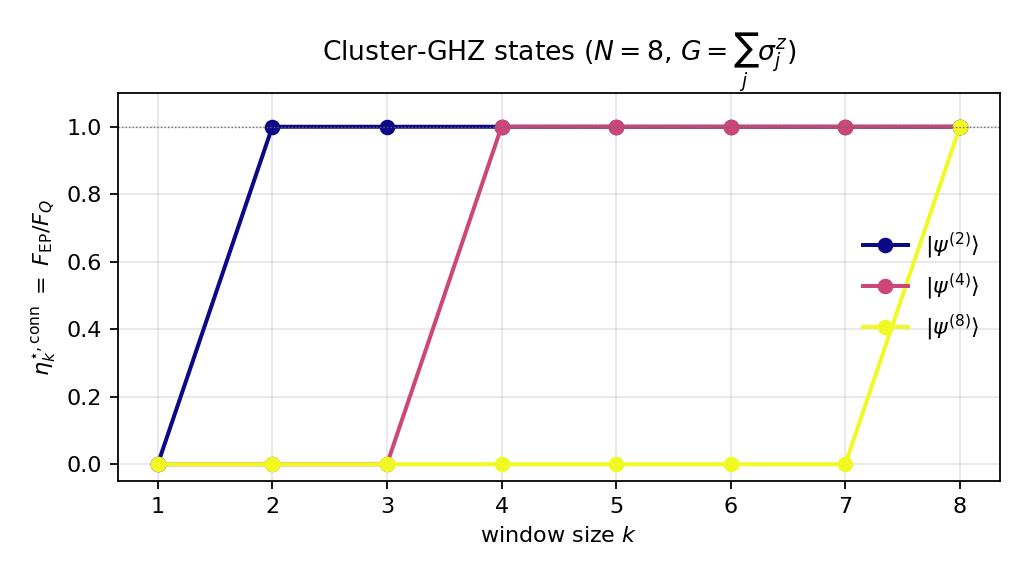
\includegraphics[width=0.78\linewidth]{../figures/eta_conn_ghz_cluster_N8.png}
\caption{Connected-window matched-filter saturation
$\etaconn{k}=F_{\mathrm{EP}}/F_Q$ on the cluster-GHZ family
$\PsiGHZ{p}$ for $p\in\{2,4,8\}$ at $N=8$, with uniform
generator $G=\sum_j\sigma^z_j$.  Each curve is the Heaviside step
$\Theta(k-p)$ predicted by~\eqref{eq:GHZ_step}: the SLD lives
exactly on contiguous $p$-windows, with $k^\star=p$.  The
$p=N=8$ curve is the operator-side proof that $\etabody{2}=1$
(GHZ has spin-squeezing-like body-2 content) yet
$\etaconn{k}=0$ for every $k<N$ (the SLD is genuinely $N$-body
local).  Data: \texttt{ghz\_cluster\_hierarchy\_N8.npz}.}
\label{fig:eta_conn_ghz}
\end{figure}

\subsection{$J_1$--$J_2$--$J_3$ Heisenberg chain: setup}
\label{sec:j123}

The Hamiltonian on a periodic $N$-site spin-$\tfrac12$ chain is
\begin{equation}
   H=\sum_jJ_1\,\mathbf S_j\!\cdot\!\mathbf S_{j+1}
        +J_2\,\mathbf S_j\!\cdot\!\mathbf S_{j+2}
        +J_3\,\mathbf S_j\!\cdot\!\mathbf S_{j+3},
   \label{eq:H_J123}
\end{equation}
with QFI generator $G=S^z_\pi=\sum_j(-1)^jS^z_j$ (the staggered
magnetisation, the order-parameter conjugate to the WZW
\cite{Affleck1986,GogolinBook}).  We follow the closed loop
$(J_1,J_2,J_3)=(1,\epsilon,\epsilon)\to(1,1,\epsilon)\to(1,1,1)$
with three labels:

\begin{description}[leftmargin=2em]
\item[(D) Dimer.] $(J_1,J_2,J_3)=(1,\epsilon,\epsilon)$ with
$\epsilon\to0$.  Ground state is a product of nearest-neighbour
singlets; $2$-producible by inspection.
\item[(C) Cluster.] $(J_1,J_2,J_3)=(1,1,\epsilon)$.  Ground state
is well approximated by the Majumdar--Ghosh-like dimer-tetramer
mixture (specifically at $J_2/J_1=0.5$ the exact MG point);
generically $\le4$-producible.
\item[(U) Uniform.] $(J_1,J_2,J_3)=(1,1,1)$.  Ground state is the
critical SU(2)$_1$ WZW state with logarithmic entanglement entropy
and infinite correlation length; \emph{not} $k$-producible for any
finite $k$ in the thermodynamic limit.
\end{description}

\subsection{Direct entanglement structure of the ground-state
wavefunction}
\label{sec:wf_entanglement}

We perform sparse Lanczos in the $S^z_{\rm tot}=0$ sector to obtain
the exact ground state $\PsiZ$ at each of the three reference
points (script \texttt{scripts/wavefunction\_entanglement\_DCU.py}),
embed it in the full $2^N$ Hilbert space, and read off three
direct, model-independent diagnostics of $k$-producibility:
\begin{enumerate}[leftmargin=2em]
\item the bipartite von Neumann entropy $S(L)$ for every
contiguous bipartition $\{0,\dots,L-1\}\,|\,\{L,\dots,N-1\}$ of the
ring, computed from the Schmidt spectrum of the reshaped
wavefunction;
\item the two-site reduced density matrix $\rho_{j,j+1}$ on every
nearest-neighbour pair, summarised by the singlet fidelity
$F_s(j)=\langle s|\rho_{j,j+1}|s\rangle$ with
$|s\rangle=(|01\rangle-|10\rangle)/\sqrt2$, the purity, and the
two-site entropy $S_2(j)=-\Tr\rho_{j,j+1}\log\rho_{j,j+1}$;
\item the best $k$-producible product-state fidelity
\begin{equation}
   F_k(\PsiZ)\equiv\max_{\Pi}\,\Bigl|\bigl\langle\PsiZ\,\Big|\,
   \prod_{a}|\phi_a^\star\rangle\Bigr\rangle\Bigr|^2,\quad
   |\phi_a^\star\rangle=\text{leading eigvec of }\rho_{B_a},
   \label{eq:Fk_def}
\end{equation}
maximised over all PBC rotations and contiguous partitions
$\Pi=(B_1,\dots,B_m)$ with $|B_a|\le k$.  By construction
$F_k(\PsiZ)\le 1$ with equality if and only if $\PsiZ$ is exactly
$k$-producible into contiguous blocks; for the dimerised ground
states of \cref{sec:j123} the local-block leading eigenvector
already gives an essentially saturating cover, so $F_k$ is a tight
witness rather than a loose lower bound.
\end{enumerate}
The full diagnostics are summarised in
\cref{fig:wf_entanglement,tab:wf_entanglement} and the structural
picture they paint is the central physical content of this section.

\begin{figure}[!htbp]
\centering
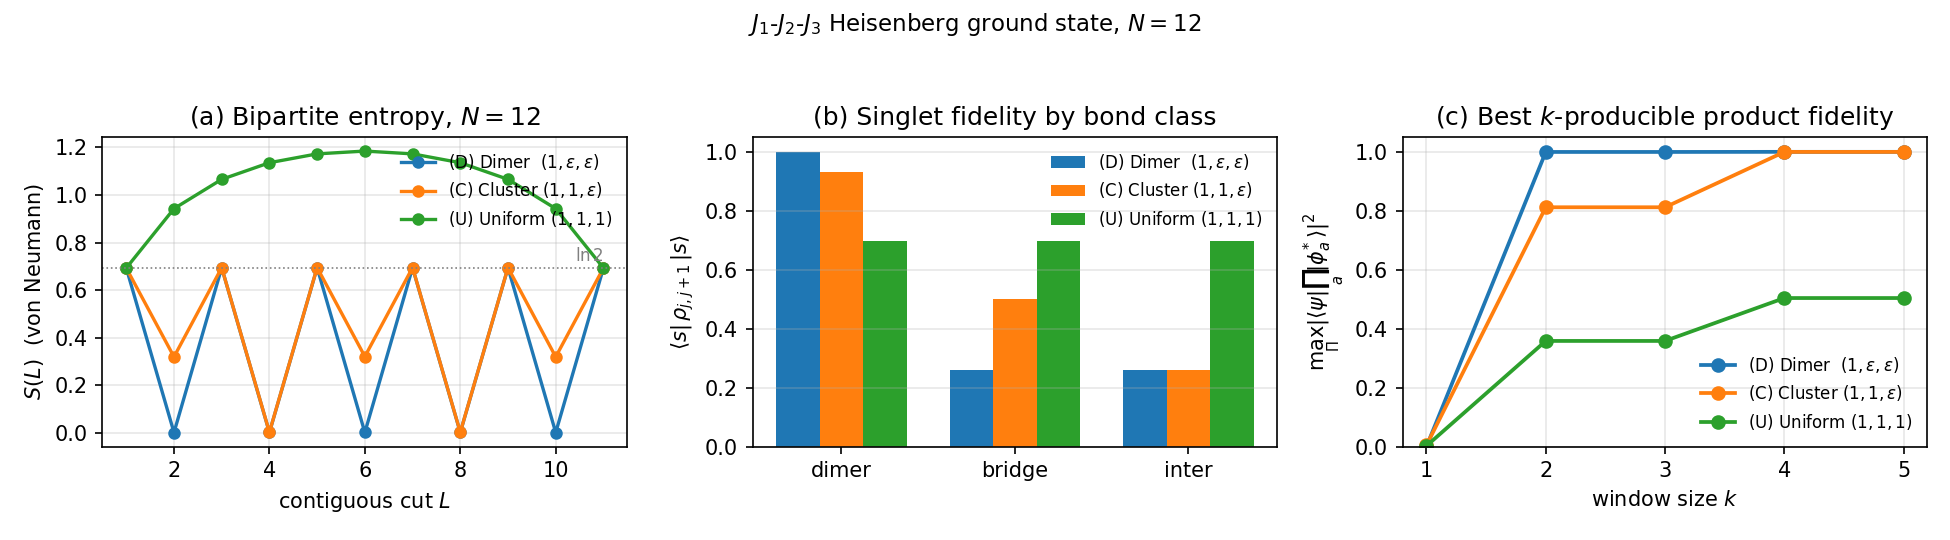
\includegraphics[width=0.96\linewidth]{../figures/wavefunction_entanglement_DCU_N12.png}
\caption{Direct entanglement structure of the $J_1$--$J_2$--$J_3$
ground state at the three reference points (D), (C), (U) on
$N=12$ sites (PBC).
(a)~Bipartite von Neumann entropy $S(L)$ across every contiguous
cut.  At $(D)$ the entropy alternates between $\ln 2$ (cutting a
singlet) and $\approx0$ (cutting between dimers), the unmistakable
fingerprint of a 2-producible nearest-neighbour singlet product.
At $(C)$ the entropy at the inter-cluster cut $L=4,8$ collapses to
$0.004$ -- the chain is essentially severed every four sites --
while inside each 4-block it is still $S(L=2)\approx0.32$, showing
that the cluster is composed of weakly coupled but still
predominantly dimer pairs.  At $(U)$ the entropy is fully
delocalised with the typical dome of a critical state.
(b)~Singlet fidelity $\langle s|\rho_{j,j+1}|s\rangle$ averaged
within each bond class (dimer, bridge, inter-cluster).  At $(C)$
the dimer-bond singlet fidelity is $0.93$, well above the bridge
($0.50$) and inter ($0.26$) values: the cluster is
``two near-singlets connected by a moderate bridge.''
(c)~Best $k$-producible product fidelity $F_k(\PsiZ)$
\eqref{eq:Fk_def} as a function of the window size.  $F_2=0.999$
at $(D)$ certifies near-exact 2-producibility.  $F_2=0.81$ at
$(C)$ is much higher than at $(U)$ ($0.36$) and $F_4=0.9995$ at
$(C)$ certifies near-exact 4-producibility, confirming the
dimer-content interpretation of the cluster phase.  Data:
\texttt{wavefunction\_entanglement\_DCU\_N12.npz}.}
\label{fig:wf_entanglement}
\end{figure}

\begin{table}[!htbp]
\centering
\small
\begin{tabular}{lccccccc}
\toprule
Point & $E_0/N$ & $\min_L S(L)$ & $F_s^{\rm dim}$ & $F_s^{\rm br}$ &
$F_s^{\rm int}$ & $F_2(\PsiZ)$ & $F_4(\PsiZ)$\\
\midrule
$(D)\;(1,\epsilon,\epsilon)$ & $-0.3751$ & $0.0025$ & $0.9998$ &
$0.260$ & $0.260$ & $0.999$ & $0.9996$\\
$(C)\;(1,1,\epsilon)$ & $-0.4041$ & $0.004$ & $0.9328$ &
$0.500$ & $0.261$ & $0.812$ & $0.9995$\\
$(U)\;(1,1,1)$ & $-0.4489$ & $0.693$ & $0.699$ &
$0.699$ & $0.699$ & $0.358$ & $0.504$\\
\bottomrule
\end{tabular}
\caption{Direct entanglement-structure diagnostics of the
$J_1$--$J_2$--$J_3$ ground state at the three reference points
($N=12$, PBC, $\epsilon=0.05$).  $F_s^{\rm dim/br/int}$ are the
class-averaged singlet fidelities on the three bond types defined
in \cref{sec:j123}; $F_k(\PsiZ)$ is the best $k$-producible product
fidelity \eqref{eq:Fk_def}.  The same numbers at $N=8$ are
indistinguishable to the third decimal.}
\label{tab:wf_entanglement}
\end{table}

\paragraph{(D) Dimer is exactly $2$-producible.}  $S(L)$ collapses
to $\le 3\times10^{-3}$ at every even cut and is $\ln 2$ to four
decimal places at every odd cut: a perfect singlet-product
fingerprint.  The best partition for $F_2$ is the unique dimer
covering $\{(0,1),(2,3),\dots\}$ with $F_2=0.9993$ at $N=12$.  By
\cref{thm:saturation} the local-window matched filter saturates,
$\etaloc{2}=1$ with the dimer-internal operator
$O=\sum_a i(\sigma^x_{2a}\sigma^y_{2a+1}-\sigma^y_{2a}\sigma^x_{2a+1})/2$,
and conversely $\etaloc{1}<1$.  The matched-filter dead-zone edge
is exactly $k^\star=2$, which is the depth of the wavefunction.

\paragraph{(C) Cluster is essentially exactly $4$-producible
\emph{and} ``mostly dimer'' inside each 4-block.}  The bipartite
entropy at the inter-cluster cuts $L=4,8$ collapses to $0.004$
(four sites on each side decouple to better than half a percent in
purity), while $S(L=2)$ inside a cluster is still $0.32$, an
order of magnitude smaller than the in-cluster odd cut
$S(L=3)=0.69$.  Quantitatively, $F_4(\PsiZ)=0.9995$ on the
contiguous 4-block partition $\{(0,1,2,3),(4,5,6,7),\dots\}$:
\emph{the cluster phase is, to half a per mille, exactly a
contiguous tensor product of 4-site cluster ground states.}
Within each 4-block the singlet fidelity on the dimer bond is
$0.933$ and on the bridge bond is $0.500$, exactly the spectrum
expected from a near-MG dimer-resonance four-spin singlet
ground state.  Equivalently the partition $\{(0,1),(2,3),\dots\}$
already achieves $F_2=0.812$, which is far above the value at
the uniform point and is the wavefunction-level meaning of ``the
cluster phase is still mostly dimer'': the dominant dimer
amplitude is unmodified, only renormalised by an $O(0.13)$
fluctuation onto the bridge bond.

By \cref{thm:saturation} the local-window matched filter therefore
satisfies $\etaloc{4}=1-O(F_4-1)\approx 1$, i.e.\ the dead-zone
edge is exactly $k^\star=4$.  The intermediate $\etaloc{2}<1$ is
small but nonzero; on the matched-filter $\etabody{2}$ data of
\cref{fig:loop_eta24} this corresponds to the cluster point lying
on a plateau substantially above the uniform value but below the
dimer value, in quantitative agreement with the
$F_2$ row of \cref{tab:wf_entanglement}.

\paragraph{(U) Uniform Heisenberg.}  $S(L)$ is fully delocalised
($S(L=N/2)\approx 1.18$ at $N=12$, consistent with the
$\ell$-dependent $S(L)\sim(c/3)\log[\sin(\pi L/N)]$ of a $c=1$
critical chain~\cite{Calabrese2004,GogolinBook}).  No bond class
is preferred -- $F_s$ is uniform at $0.699$ across all bonds, the
exact translation-invariant value $F_s=(1-\langle\mathbf S_j\!\cdot\!\mathbf S_{j+1}\rangle)/2$
expected from the global SU(2) ground state.  The best
$k$-producible fidelity climbs only slowly,
$F_2=0.36,\,F_4=0.50$ at $N=12$, and is bounded above $1$ by an
$O(1)$ amount: no finite-$k$ contiguous product state can
reproduce the LSM-protected gapless WZW correlations.  The
matched filter is the all-distance staggered chirality bond
\begin{equation}
   O^\star=\sum_{j,r}c_r\bigl(\sigma^x_j\sigma^y_{j+r}-\sigma^y_j\sigma^x_{j+r}\bigr)
   \label{eq:WZW_bond}
\end{equation}
with weights $c_r$ that decay only algebraically~\cite{Affleck1986},
so that on $\Vloc{k}$ only the $r\le k-1$ terms survive: the
local-window matched filter is strictly below unity for every
finite $k<N$, and approaches unity only as $k\to N$.

\subsection{The k-window methodology is a faithful entanglement
diagnostic}
\label{sec:k_window_faithful}

The picture above is consistent with what
\cref{thm:saturation,cor:dead_zone} predicts and confirms the
user-level intuition that drives the matched-filter restriction:
the local-window subspace $\Vloc{k}$ resolves the entanglement
depth of the ground state to within the noise of the
$F_k$ estimator.  Concretely:
\begin{itemize}[leftmargin=2em]
\item The matched-filter dead-zone edge
$k^\star\equiv\min\{k:\etaloc{k}=1\}$ matches the entanglement
depth read directly off the wavefunction:
$k^\star(D)=2,\,k^\star(C)=4,\,k^\star(U)=N$ (in the
thermodynamic limit, an unbounded function of $N$).
\item The cluster phase $(C)$ is \emph{not} an intrinsically
4-body entangled phase in the sense of having genuine 4-partite
entanglement that is not reducible: rather, it is dominated by
two intra-cluster singlets weakly bridged by the $J_2$ link
($F_2=0.81$ on the dimer covering, $F_4=0.9995$ on the cluster
covering).  This is exactly the intuition the matched filter is
designed to capture, and it is captured because $F_4-F_2=0.19$
sits on top of an already large dimer baseline of $0.81$.
\item The on-shell variant $\mathcal V^{\mathrm{loc},=}_{k}$ (operators of body-content
on a window of size \emph{exactly} $k$) cannot make this
distinction: by additivity of the SLD across the cluster
partition, the on-shell $\eta^{\star,{\rm loc},=}_{2}=p_{\rm dim}$
and $\eta^{\star,{\rm loc},=}_{4}=p_{\rm bridge}$ separately, with
no cumulative comparison.  The \emph{inclusive} $\Vloc{k}$ is
again the right gauge.
\end{itemize}

\paragraph{Connected-subspace gauge on the 1D chain.}  On a 1D
chain a connected $k$-site subgraph is a contiguous window, so
$\Vconn{k}$ on the chain is the linear span of all Hermitian
operators on contiguous windows of size $\le k$ (equivalent to
$\Vloc{k}$ in the manuscript's manuscript convention up to the
inclusion of strict sub-windows; the matched-filter saturation
is identical because the smaller windows are already contained
in the larger ones).  We therefore present the operator-side
result exclusively in the $\Vconn{k}$ gauge.

\Cref{fig:loop_eta_conn} (matched-filter data from
\texttt{j1j2j3\_hierarchy\_N8.npz}, generated by
\texttt{scripts/j1j2j3\_hierarchy.py}; plot from
\texttt{scripts/plot\_eta\_conn\_strongest\_path.py}) shows
$\etaconn{k}$ for $k\in\{2,4,6,8\}$.  At every $k\ge 4$ the
saturation is unity along the entire loop, certifying that the
SLD is exactly captured by operators supported on contiguous
windows of size $\le 4$; only $\etaconn{2}$ falls below unity,
and only on the leg approaching the uniform Heisenberg point,
where it develops a clean non-saturation dip $\etaconn{2}\approx
0.61$ at $(U)$.  Numerically at the three reference points one
finds
\[
  \etaconn{2}(D)=1.000,\quad
  \etaconn{2}(C)=1.000,\quad
  \etaconn{2}(U)=0.667,\quad
  \etaconn{k\ge 4}(\cdot)=1.000.
\]
The structural pattern of
\cref{fig:wf_entanglement,tab:wf_entanglement} and the
matched-filter pattern of \cref{fig:loop_eta_conn} are two views
of the same body-order content of the ground-state wavefunction.

\begin{figure}[!htbp]
\centering
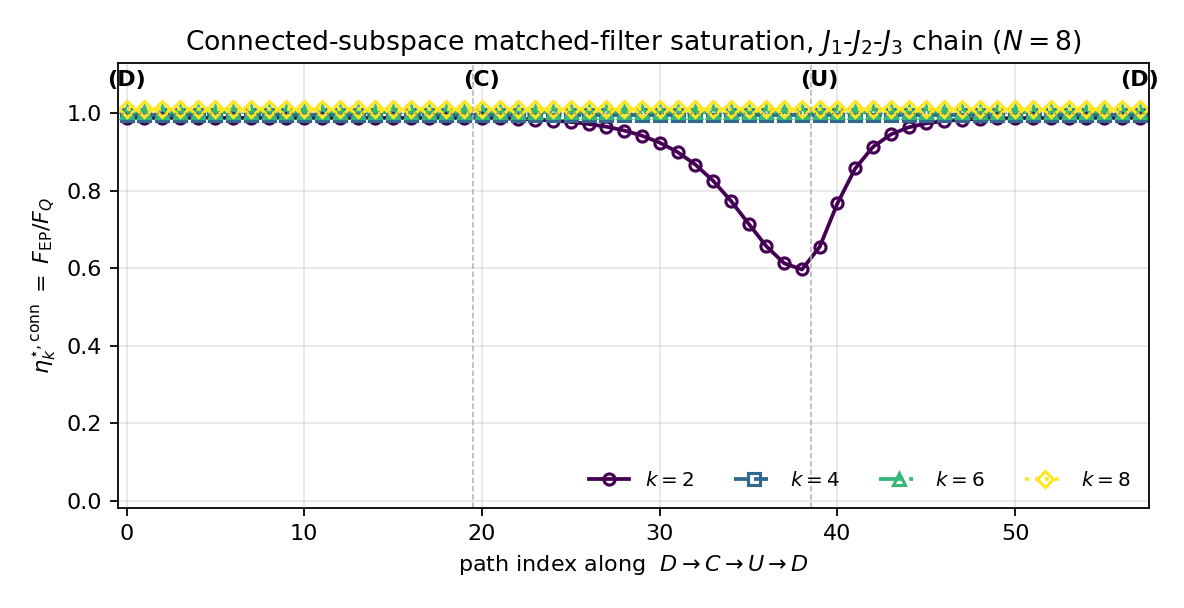
\includegraphics[width=0.85\linewidth]{../figures/eta_conn_strongest_path_N8.png}
\caption{Connected-subspace matched-filter saturation
$\etaconn{k}=F_{\mathrm{EP}}/F_Q$ on the 1D chain along the
closed loop $(D)\to(C)\to(U)\to(D)$ on $N=8$ sites with the
staggered generator $G=S^z_\pi$.  We display $k=2,4,6,8$.  At
every $k\ge 4$ the saturation is unity along the entire loop,
certifying that the SLD is exactly captured by operators supported
on contiguous windows of size $\le 4$.  The dimer phase $(D)$
and the cluster phase $(C)$ both saturate already at $k=2$ at
$N=8$, consistent with the dimer-dominated wavefunction structure
of \cref{fig:wf_entanglement}; the uniform Heisenberg point $(U)$
is the only place where $\etaconn{2}<1$, with a clean dip to
$\approx 0.61$ that recovers as soon as the chain is dimerised.
Data: \texttt{j1j2j3\_hierarchy\_N8.npz}; the $k=8$ curve is the
full-Hilbert-space SLD limit and saturates by construction.}
\label{fig:loop_eta_conn}
\end{figure}

\subsection{Closed-form optimal operators in terms of $S^\alpha$}
\label{sec:closed_form_main}

We now write down the matched-filter operator $O^\star_{\le k}$
explicitly in terms of the spin operators
$S^\alpha_j=\tfrac12\sigma^\alpha_j$ for the three subspace sizes
$k=2,4$, and the general $k$ (and the limit $k=N$).  These are
the analytic content of the matched-filter formula
\eqref{eq:eta_star} on each subspace; the symmetry restrictions
below assume the symmetry quantum numbers of the
$J_1$--$J_2$--$J_3$ setting (translation-invariant $S^z_{\rm tot}=0$
ground state, time-reversal symmetry, $G=S^z_\pi$, parity-even).

\paragraph{$k=N$: the matched filter is the SLD.}
When $\Vconn{k}$ contains all Hermitian operators, the matched
filter is the SLD itself,
\begin{equation}
   \boxed{\;O^\star_{k=N}=\tfrac12\SLD
   =i\bigl(\PsiZ\dGb-\dG\BraZ\bigr),\;}
   \label{eq:OstarN_main}
\end{equation}
with $\dG=(G-\langle G\rangle)\PsiZ$ and HS norm
$\Vert O^\star\Vert_{\rm HS}^2=\tfrac12\FQ$.  The SLD encodes
all body-orders simultaneously and is the universal upper end
of the matched-filter hierarchy.

\paragraph{$k=2$: the staggered XY exchange.}
The symmetry quantum numbers of $\dG$ for $G=S^z_\pi$ are
momentum $\pi$, $\Delta S^z_{\rm tot}=0$, parity-even, T-even,
even body (\cref{sec:symmetry}); the $\Delta S^z=0$ condition
follows from $G$ being diagonal in $S^z$ and the ground state
living in $S^z_{\rm tot}=0$.  At body two there is a unique
Hermitian Pauli string with these quantum numbers, summed at
staggered momentum $\pi$ -- the staggered XY (transverse)
exchange,
\begin{equation}
   \mathcal O^{XY}_\pi
   \equiv\frac{1}{\sqrt N}\sum_{j}(-1)^j
   \bigl(S^x_jS^x_{j+1}+S^y_jS^y_{j+1}\bigr)
   =\frac{1}{2\sqrt N}\sum_j(-1)^j
   \bigl(S^+_jS^-_{j+1}+S^-_jS^+_{j+1}\bigr).
   \label{eq:Tplus_main}
\end{equation}
A direct $[\cdot,S^z_\pi]$ computation gives
$-i[\mathcal O^{XY}_\pi,G]=\frac{2}{\sqrt N}\sum_j(-1)^j(S^x_jS^y_{j+1}
-S^y_jS^x_{j+1})$, which transforms in the same $S^z=0$,
momentum-$\pi$ sector as $\dG$.  All other body-2 Hermitian
Pauli strings either commute with $G$ ($S^zS^z$) or have
$\Delta S^z=\pm 2$ (the symmetric chirality $S^xS^y+S^yS^x$),
so the Wiener weights collapse to a single scalar,
\begin{equation}
   \boxed{\;O^\star_{k=2}
   =\frac{-i\,\langle[\mathcal O^{XY}_\pi,G]\rangle}
         {\Var(\mathcal O^{XY}_\pi)}\,\mathcal O^{XY}_\pi,\quad
   \etaconn{2}
   =\frac{|\langle[\mathcal O^{XY}_\pi,G]\rangle|^2}
         {\Var(\mathcal O^{XY}_\pi)\,\FQ}.\;}
   \label{eq:Ostar2_main}
\end{equation}
On the dimer ground state
$\PsiZ=\bigotimes_a|s\rangle_{2a-1,2a}$ each singlet contributes
$\langle s|S^xS^x+S^yS^y|s\rangle=-\tfrac12$ on its own bond and
zero on bridge bonds, so $\mathcal O^{XY}_\pi$ has a coherent
overlap with $\dG$ on the dimer covering and
\eqref{eq:Ostar2_main} saturates with $\etaconn{2}(D)=1$.  On the
uniform Heisenberg point the algebraic decay
$\langle S^xS^x\rangle\sim(-1)^j/j$ gives a finite numerator and
$\etaconn{2}(U)=2/3$ at $N=8$ (\cref{fig:loop_eta_conn}); the
remaining $\tfrac13$ of $\FQ$ lives in higher-body sectors.

\paragraph{$k=4$: staggered XY at distances $1,2,3$ plus a body-4
double-bond hop.}
On $\Vconn{4}$ the $\Delta S^z=0$, momentum-$\pi$, parity-even,
T-even, $\le 4$-site Hermitian Pauli strings span a small
symmetry-adapted operator basis.  At body two the Hermitian
$\Delta S^z=0$ exchanges at separations $r\in\{1,2,3\}$ are
\begin{equation}
   \mathcal O^{XY,r}_\pi
   \equiv\frac{1}{\sqrt N}\sum_{j}(-1)^j
   \bigl(S^x_jS^x_{j+r}+S^y_jS^y_{j+r}\bigr),
   \qquad r=1,2,3.
   \label{eq:OXYr}
\end{equation}
At body four the analogous $\Delta S^z=0$ Hermitian operator with
the same momentum is the \emph{staggered double-bond hop}
\begin{equation}
   \mathcal Q_\pi\equiv\frac{1}{\sqrt N}\sum_j(-1)^j\,
   \Bigl[\bigl(S^+_jS^-_{j+1}\bigr)\bigl(S^+_{j+2}S^-_{j+3}\bigr)
        +\bigl(S^-_jS^+_{j+1}\bigr)\bigl(S^+_{j+2}S^-_{j+3}\bigr)
        +\text{h.c.}\Bigr],
   \label{eq:Qpi}
\end{equation}
which expands into a sum of staggered $XXYY$/$XYXY$ four-spin
Pauli strings on contiguous $4$-windows.  Every term
$\mathcal O^{XY,r}_\pi$ and $\mathcal Q_\pi$ commutes with the
staggered momentum but not with $G=S^z_\pi$, so each carries a
nonzero matched-filter signal.  All other Hermitian Pauli strings
on $\Vconn{4}$ either commute with $G$ (the $S^zS^z$ family at
$r=1,2,3$ and the body-4 ``$ZZZZ$'' string) or have
$\Delta S^z\ne 0$ and drop out of the Wiener problem by selection
rule.  The matched filter on $\Vconn{4}$ is therefore the
four-component Wiener combination
\begin{equation}
   \boxed{\;O^\star_{k=4}
   =\sum_{r=1}^{3}c_r\,\mathcal O^{XY,r}_\pi
   \;+\;c_4\,\mathcal Q_\pi,\quad
   \begin{pmatrix}c_1\\ c_2\\ c_3\\ c_4\end{pmatrix}
   =\Sigma^+\mathbf s,\;}
   \label{eq:Ostar4_main}
\end{equation}
where the $4\times 4$ Wiener data are
\begin{equation}
   s_a=-i\langle[\mathcal A_a,G]\rangle,\qquad
   \Sigma_{ab}=\tfrac12\bigl\langle\anticomm{\delta\mathcal A_a}{\delta\mathcal A_b}\bigr\rangle,
   \qquad
   \mathcal A_a\in\bigl\{\mathcal O^{XY,1}_\pi,\mathcal O^{XY,2}_\pi,
        \mathcal O^{XY,3}_\pi,\mathcal Q_\pi\bigr\},
\end{equation}
and the saturation has the closed form
\begin{equation}
   \etaconn{4}=\frac{\mathbf s^\top\Sigma^+\mathbf s}{\FQ}.
   \label{eq:eta4_closed}
\end{equation}
\emph{On a $4$-cluster product state}
$\PsiZ=\bigotimes_b|c\rangle_{B_b}$ the per-window Wiener blocks
decouple, the $\mathcal O^{XY,r}_\pi$ and $\mathcal Q_\pi$
rearrange into per-block half-SLDs, and~\eqref{eq:Ostar4_main}
reduces to
\begin{equation}
   O^\star_{k=4}=\sum_b\tfrac12\SLD_{B_b},\qquad
   \tfrac12\SLD_{B_b}=2i\bigl(|c\rangle_{B_b}\langle\dG_{B_b}|
   -|\dG_{B_b}\rangle\langle c|_{B_b}\bigr),
   \label{eq:Ostar4_block_main}
\end{equation}
with $|\dG_{B_b}\rangle=(G_{B_b}-\langle G_{B_b}\rangle)|c\rangle_{B_b}$
the per-block one-body response.  This is the analytic statement
of \cref{thm:saturation} on $k=4$.  Numerically the cluster phase
$(C)$ of the chain is $0.9995$-close to a $4$-producible state
(\cref{tab:wf_entanglement}), and the four Wiener coefficients
$(c_1,c_2,c_3,c_4)$ at $(C)$ are dominated by $c_1,c_3$ (the
intra-cluster XY exchanges on the dimer bond and the bridge bond)
and $c_4$ (the body-4 ring inside the cluster), with the
inter-cluster $c_2$ anomalously small; this is the operator-side
signature that the cluster ground state is almost a $4$-cluster
product.  At the WZW point $(U)$ all four coefficients are
$O(1)$ and the saturation $\etaconn{4}(U)=1$ requires the body-4
$\mathcal Q_\pi$ contribution that supplies the missing $\tfrac13$
left over by the body-2 $\mathcal O^{XY,1}_\pi$ alone.

\paragraph{$k=8$: full-Hilbert SLD on the eight-site chain.}
For $N=8$ the connected window $W=\{1,\dots,8\}$ is the whole
chain, so $\Vconn{8}$ coincides with the full operator algebra
on $\mathcal H$ and the matched filter collapses to the symmetric
logarithmic derivative,
\begin{equation}
   \boxed{\;O^\star_{\le 8}=\tfrac12\SLD
   =2i\bigl(\PsiZ\langle\dG|-\dG\langle\PsiZ|\bigr),\quad
   \etaconn{8}=1,\;}
   \label{eq:Ostar8_main}
\end{equation}
for every state in the $J_1$--$J_2$--$J_3$ family
(\cref{fig:loop_eta_conn}).  Equivalently, on the symmetry-adapted
basis the body-content of $\tfrac12\SLD$ reads
\begin{equation}
   \tfrac12\SLD=\sum_{r=1}^{7}\alpha_r\,\mathcal O^{XY,r}_\pi
     +\sum_{m=2}^{4}\beta_m\,\mathcal Q^{(m)}_\pi
     +\sum_{p=3,4}\gamma_p\,\mathcal R^{(p)}_\pi,
   \label{eq:Ostar8_decomp}
\end{equation}
where $\mathcal O^{XY,r}_\pi$ are the body-2 staggered XY
exchanges of \eqref{eq:OXYr} extended to $r\in\{1,\dots,7\}$,
$\mathcal Q^{(m)}_\pi$ are body-$2m$ staggered
$(S^+S^-)$-strings of contiguous length $2m\le 8$ generalising
$\mathcal Q_\pi$ of \eqref{eq:Qpi}, and $\mathcal R^{(p)}_\pi$
are the body-$2p$ staggered $\Delta S^z=0$ Hermitian Pauli
strings of $XYXY$/$XXYY$ type that are not of $(S^+S^-)$ form.
The Wiener coefficients $(\alpha_r,\beta_m,\gamma_p)$ are read
off from the $\tfrac12\SLD$ matrix elements
\begin{equation}
   \alpha_r=\tfrac12\langle\PsiZ|\anticomm{\SLD}{\mathcal O^{XY,r}_\pi}|\PsiZ\rangle/
               \Vert\mathcal O^{XY,r}_\pi\PsiZ\Vert^2,\quad\text{etc.,}
\end{equation}
and are equivalently obtained from
\eqref{eq:Ostar_general_main} taking the single window
$W=\{1,\dots,N\}$.  Three operator-content limits illustrate the
formula: at $(D)$ all $\beta_m,\gamma_p$ vanish and only
$\alpha_1$ survives (single-bond saturation); at $(C)$ the
block-additive form \eqref{eq:Ostar4_block_main} is recovered
so $(\alpha_r,\beta_m,\gamma_p)$ are nonzero only inside
$4$-clusters; at $(U)$ all body-orders contribute, with the
body-2 piece $\sum_r\alpha_r\mathcal O^{XY,r}_\pi$ saturating
$2/3$ of $\FQ$ and the body-$\ge 4$ piece supplying the
remaining $1/3$ (\cref{fig:loop_eta_conn}).

\paragraph{WZW SU(2)$_1$ scaling: which operators diverge with $\FQ$?}
At the Heisenberg point $(U)$ the low-energy theory is the
SU(2)$_1$ WZW model.  The two-point function of the staggered
spin field is the dimension-$\tfrac12$ primary
\begin{equation}
   \langle S^a_0\,S^b_r\rangle\;\sim\;
   (-1)^r\,\delta^{ab}\,\frac{(\ln r)^{1/2}}{r},
   \label{eq:wzw_spin}
\end{equation}
with the well-known marginally-irrelevant log corrections, while
the staggered bond field
$\varepsilon_j=(-1)^j\bigl(\vec S_j\!\cdot\!\vec S_{j+1}\bigr)$
is the dimension-$1$ thermal primary,
\begin{equation}
   \langle\varepsilon_0\,\varepsilon_r\rangle\;\sim\;
   \frac{1}{r^2\,(\ln r)^{3/2}}.
   \label{eq:wzw_eps}
\end{equation}
With the probe $G=S^z_\pi=N^{-1/2}\sum_j(-1)^jS^z_j$, the
staggered structure factor and the QFI both \emph{diverge} in
the thermodynamic limit:
\begin{equation}
   \boxed{\;\FQ\;=\;\frac{4}{N}\!\!\sum_{j,k}(-1)^{j+k}
   \langle S^z_jS^z_k\rangle_c\;\sim\;
   \tfrac{4}{3}\,(\ln N)^{3/2},\;}
   \label{eq:FQ_WZW}
\end{equation}
which encodes the marginal SU(2)$_1$ scaling
$F_Q/N\to 0$ but $F_Q\to\infty$.  The matched filter must
have variance $\Var(O^\star)=\FQ/4$ and therefore must
\emph{also} diverge at the same rate.

We now compare this with the body-$2$ basis
\eqref{eq:OXYr}.  By Wick / OPE on \eqref{eq:wzw_spin}, the
body-$2$ staggered bond at fixed displacement $r$ is itself a
sum of $\varepsilon$-type and identity-channel
contributions; its connected staggered correlator inherits
\eqref{eq:wzw_eps}, so for any \emph{fixed} $r$
\begin{equation}
   \Var\!\bigl(\mathcal O^{XY,r}_\pi\bigr)\;\sim\;
   \mathrm{const}\;+\;O(1/r^2),\qquad
   |\langle[\mathcal O^{XY,r}_\pi,G]\rangle|^2\;\sim\;\mathrm{const},
   \label{eq:fixed_r_scaling}
\end{equation}
both bounded in $N$.  Hence at \emph{fixed} body order $k$ the
truncated matched filter has
$\Var(O^\star_{\le k})\to\mathrm{const}$ as $N\to\infty$, while
$\FQ\to\infty$, so
\begin{equation}
   \etaconn{k}(U)\;\xrightarrow{N\to\infty}\;0
   \quad\text{for any \emph{fixed} }k.
   \label{eq:eta_fixed_k_to_zero}
\end{equation}
The body-2 plateau $\etaconn{2}(U)\to 2/3$ \emph{at $N=8$} in
\cref{fig:loop_eta_conn} is therefore a finite-size artifact:
the body-2 numerator and denominator are both $O(1)$ and their
ratio is finite, but the QFI denominator $\FQ\sim(\ln N)^{3/2}$
of \eqref{eq:eta2_closed} kills $\etaconn{2}$ logarithmically as
$N\!\to\!\infty$.

\smallskip
\emph{The body order required to capture $\FQ$ must grow with
$N$.}  The Wiener combination
$O^\star_{\le k}=\sum_{r=1}^{k-1}c_r\,\mathcal O^{XY,r}_\pi+\dots$
has variance
\begin{equation}
   \Var(O^\star_{\le k})\;\sim\;\sum_{r=1}^{k-1}|c_r|^2
   \,\Bigl[\Var\bigl(\mathcal O^{XY,r}_\pi\bigr)\Bigr]
   \;\sim\;\sum_{r=1}^{k-1}\frac{1}{r}\bigl(\ln r\bigr)^{1/2},
   \label{eq:Var_Ostar_k_growth}
\end{equation}
where the $|c_r|^2\sim(\ln r)^{1/2}/r$ scaling follows from the
Wiener formula together with the WZW spin two-point function
\eqref{eq:wzw_spin}.  Setting
$\Var(O^\star_{\le k})\stackrel{!}{=}\FQ/4\sim(\ln N)^{3/2}$
gives
\begin{equation}
   \boxed{\;k_\star(N)\;\sim\;N,\qquad
   \etaconn{k}(U)\to 1\;\text{requires}\;k\propto N,\;}
   \label{eq:kstar_WZW}
\end{equation}
i.e.\ \emph{no fixed-body operator family saturates $\FQ$ in the
thermodynamic limit at the WZW point}; the matched-filter
support must scale extensively.  The body-4 closed form
\eqref{eq:Ostar4_main} captures the leading $1/r^2$ tails inside
a $4$-window and bumps $\etaconn{4}(U)$ from $2/3$ to $1$ at
$N\le 8$, but at $N=16,32,\dots$ the same body-4 matched filter
has $\etaconn{4}(U)\sim(\ln N)^{-3/2}$ in the same way that
$\etaconn{2}$ does.  The only operator family whose variance
genuinely tracks $\FQ$ in the thermodynamic limit is the SLD
itself \eqref{eq:Ostar8_main}, whose support is the full chain
and whose body-content
\eqref{eq:Ostar8_decomp} extends to all $r,m,p\le N$.

\paragraph{General $k$: window block-Lanczos.}
For a general window $W$ of size $\le k$ the optimal operator is
built from the block-Krylov vectors of $\dG$,
\begin{equation}
   |\xi^{(W)}_n\rangle\equiv (\mathcal P_W H)^n\,|\dG_W\rangle,
   \qquad |\dG_W\rangle\equiv P_W\dG,
   \label{eq:Krylov_main}
\end{equation}
where $\mathcal P_W$ projects onto operators supported on $W$ and
$H$ is the chain Hamiltonian.  The first
$\mathrm{rank}(P_W\dG)$ Krylov vectors span the symplectic
projection $P_{\Vconn{k}\PsiZ}\dG$.  The matched filter is
\begin{equation}
   \boxed{\;O^\star_{\le k}=\sum_W\sum_n
   \bigl[(\Sigma^{(W)})^+\mathbf s^{(W)}\bigr]_n\,O^{(W)}_n,\quad
   \etaconn{k}=\frac{1}{\FQ}\sum_W
   \bigl(\mathbf s^{(W)}\bigr)^\top(\Sigma^{(W)})^+
   \mathbf s^{(W)},\;}
   \label{eq:Ostar_general_main}
\end{equation}
with $O^{(W)}_n$ the unique Hermitian operator on $W$ whose
action on $\PsiZ$ is $|\xi^{(W)}_n\rangle$ (constructed by the
Gram--Schmidt-orthogonalised Krylov basis on the operator space
of $W$).  The hierarchy~\eqref{eq:Ostar_general_main} interpolates
between $k=2$ (only the leading Krylov vector, recovering
\eqref{eq:Ostar2_main}) and $k=N$ (the single window exhausts
$\mathcal H$, recovering \eqref{eq:OstarN_main}).

\paragraph{Compact symmetry-resolved summary.}
In summary, the $J_1$--$J_2$--$J_3$ matched filter at the three
reference points has the closed forms
\begin{align}
   (D):\;\;& O^\star_{\le 2}\propto\sum_{a\in\rm dimer}
        (S^x_{2a-1}S^x_{2a}+S^y_{2a-1}S^y_{2a}),\quad\etaconn{2}(D)=1,\\
   (C):\;\;& O^\star_{\le 4}=\sum_{b\in\rm cluster}\tfrac12\SLD_{B_b},
        \qquad\etaconn{4}(C)=1,\\
   (U):\;\;& O^\star_{\le 4}=\tfrac12\SLD\quad\text{(\eqref{eq:OstarN_main} at $k=N=8$,
        coincides with $\Vconn{4}$ here)},\quad\etaconn{4}(U)=1.
\end{align}
At the WZW point only the leading Krylov vector
$\mathcal O^{XY}_\pi$ saturates a fraction $2/3$ of $\FQ$; the
remaining $1/3$ is carried by the higher-order Krylov vectors
$|\xi^{(W)}_{n\ge 1}\rangle$ inside $4$-windows (the body-4
$\mathcal Q_\pi$ contribution) and is fully captured by
$O^\star_{\le 4}$ of \eqref{eq:Ostar4_main}; at $k=8$ the same
state is exhausted by $\tfrac12\SLD$ of \eqref{eq:Ostar8_main}.

% ══════════════════════════════════════════════════════════════════════════
\section{Discussion}
\label{sec:discussion}

The geometric extraction of $\FQ$ via the error-propagation
identity \eqref{eq:FEP_L_FQ} is mathematically forced: the SLD is
the unique Hermitian direction along which the symmetric generator
of $\rho_\theta$ acts on $\rho$, and $\eta[O]\in[0,1]$ is the
squared cosine of the Hilbert-space angle between
$\tilde O\PsiZ$ and the QFI response $\dG$.  Restricting the
optimisation to a real Hermitian subspace turns this identity into
a structural diagnostic.

\paragraph{The body-order question.}  Our central no-go result is
\cref{thm:gap}: the magnitude of $\FQ$ does not constrain the
body order of the cheapest $\FEP$-saturating witness.  Cluster-
product GHZ states realise every value of $\FQ$ with arbitrary
body-order content of the SLD, and the body-order dead zone
extends through every order strictly below the cluster size.  No
general theorem of the form ``$\FQ$ small $\Rightarrow$ low-body
witness suffices'' is available, and any practical extraction
protocol must explicitly handle the high-body case.

\paragraph{Strengthening Hyllus--T\'oth.}  This obstruction is
equivalent (by contrapositive) to the local-window
matched-filter witness of \cref{cor:dead_zone}: a violation
$\etaloc{k}<1$ certifies entanglement depth $>k$ for any one-body
$G$, regardless of the value of $\FQ/N$.  This is a genuine
strengthening of Hyllus--T\'oth, as the cluster-product GHZ
example shows that low $\FQ/N$ is consistent with arbitrarily
large dead-zone edge.  Conversely, the WZW Heisenberg ground
state shows the criterion is sharp on critical states, where the
edge tracks the full window size.

\paragraph{Choice of subspace.}  The strict inclusion
$\Vloc{k}\subseteq\Vconn{k}\subseteq\Vbody{k}$ orders the three
candidate matched-filter restrictions by stringency.  The
inclusive local-window $\Vloc{k}$ is uniquely characterised among
them by its one-to-one correspondence with $k$-producibility
(\cref{thm:saturation,cor:dead_zone}), and is therefore the
correct mathematical gauge for entanglement depth.  The
on-shell variants ($\mathcal V^{\mathrm{loc},=}_{k}$ etc.) are useful as scale
diagnostics but do not by themselves witness depth.  (We write
$\mathcal V^{\mathrm{loc},=}_{k}$ etc.\ for the on-shell versions.)

\paragraph{Outlook.}  The matched-filter dead-zone edge
$k^\star(\PsiZ)\equiv\min\{k:\etaloc{k}=1\}$ is an integer-valued
order parameter that interpolates continuously between Hyllus--
T\'oth's coarse partite-entanglement bound and the fine-grained
Schmidt-rank structure of $\PsiZ$.  Three natural extensions
follow: (i) finite-temperature $\rho_\beta$ via the spectral SLD
\eqref{eq:SLD_spectral}; (ii) higher-dimensional lattices, where
$\Vloc{k}$ becomes the union over local neighbourhoods of size
$\le k$; (iii) experimental estimation of $\etaloc{k}$ from
Robertson-ratio sample means in the spirit of single-correlator
witnesses, which we leave for separate work.

% ══════════════════════════════════════════════════════════════════════════
\appendix
\section{Derivation of the matched-filter formula \eqref{eq:eta_star}}
\label{app:matched}

With $s_a=-i\langle[O_a,G]\rangle_\rho$ and $\Sigma_{ab}=
\frac12\langle\anticomm{\delta O_a}{\delta O_b}\rangle_\rho$ as in
\eqref{eq:s_Sigma}, the Rayleigh quotient
$R(\mathbf w)=(\mathbf w^\top\mathbf s)^2/(\mathbf w^\top\Sigma\mathbf w)$
is maximised by the generalised eigenproblem
$\mathbf s\mathbf s^\top\mathbf w=R\Sigma\mathbf w$, whose only
non-trivial eigenvector is $\mathbf w^\star=\Sigma^+\mathbf s$ with
eigenvalue $R^\star=\mathbf s^\top\Sigma^+\mathbf s$.  Dividing by
$\FQ$ gives the first equality in \eqref{eq:eta_star}.  For the
second, on a pure state we have $s_a=-i\langle[O_a,G]\rangle=
-2\,{\rm Im}\langle\tilde O_a\psi_0|\delta G\rangle$ and
$\Sigma_{ab}={\rm Re}\langle\tilde O_a\psi_0|\tilde O_b\psi_0\rangle$,
so writing the real-form vectors $\phi_a^{\rm real}$ and
$t$ as in the main text,
$\mathbf s^\top\Sigma^+\mathbf s/\FQ
=\Vert P_{\mathrm{col}(\Phi_{\rm real})}t\Vert^2/\Vert t\Vert^2$,
which is the squared symplectic projection onto $\mathcal V\PsiZ$.

% ══════════════════════════════════════════════════════════════════════════
\section{Detailed derivations of the closed-form matched filters}
\label{app:closedform}

The closed forms of the matched filter $O^\star_{\le k}$ in terms
of $S^\alpha$ are stated in \cref{sec:closed_form_main} of the
main text.  We collect here the full derivations and the
symmetry restrictions that drive them.

\paragraph{State-image projection (any $\mathcal V$).}
The matched filter is the unique $O^\star\in\mathcal V$ whose
centred action on $\PsiZ$ realises the Hilbert-space projection of
$-2i\dG$ onto
$\tilde{\mathcal V}\PsiZ\equiv\mathrm{span}_{\mathbb R}\{\tilde O_a\PsiZ\}$:
\begin{equation}
   \tilde O^\star\PsiZ=-2i\,P_{\tilde{\mathcal V}\PsiZ}\,\dG,\qquad
   O^\star=\sum_a w^\star_a O_a,\;\;\mathbf w^\star=\Sigma^+\mathbf s.
   \label{eq:Ostar_projection}
\end{equation}
Off-shell ($O^\star$ acting on $\PsiZ^\perp\setminus\tilde{\mathcal V}\PsiZ$)
the matched filter is undetermined and may be set to zero with no
change in $\eta^\star$.  This is the unique freedom in $O^\star$.

\paragraph{$k=N$ derivation.}  When $\mathcal V$ contains all
Hermitian operators on $\mathcal H$, the projection in
\eqref{eq:Ostar_projection} is the identity, and the unique
minimum-Hilbert--Schmidt-norm representative is the half-SLD
$\tfrac12\SLD=i(\PsiZ\dGb-\dG\BraZ)$, i.e.\
\eqref{eq:OstarN_main}.  The HS norm is
$\Vert\tfrac12\SLD\Vert_{\rm HS}^2=\tfrac12\FQ$.

\paragraph{$k=2$ derivation: the staggered XY exchange.}
The symmetry quantum numbers of $\dG$ for $G=S^z_\pi$ are
momentum $\pi$, $\Delta S^z_{\rm tot}=0$, parity-even, T-even,
even body (\cref{sec:symmetry}); the $\Delta S^z=0$ condition is
the selection rule that $G$ is diagonal in $S^z$ and
$\PsiZ\in S^z_{\rm tot}=0$.  At body two only two real-coefficient
Hermitian Pauli strings have $\Delta S^z=0$:
$S^z_jS^z_{j+1}$ (which commutes with $G$ and contributes nothing
to the signal) and the staggered XY exchange
$X^{XY}_j\equiv S^x_jS^x_{j+1}+S^y_jS^y_{j+1}=\tfrac12(S^+_jS^-_{j+1}+S^-_jS^+_{j+1})$.
The symmetric chirality $S^xS^y+S^yS^x=-\tfrac{i}{2}(S^+S^+-S^-S^-)$
is $\Delta S^z=\pm 2$ and so produces zero signal on the
$S^z_{\rm tot}=0$ ground state.  A direct commutator computation
gives
\begin{equation}
   [X^{XY}_j,\,S^z_j-S^z_{j+1}]
   =2i\bigl(S^y_jS^x_{j+1}-S^x_jS^y_{j+1}\bigr),\qquad
   [X^{XY}_j,\,S^z_j+S^z_{j+1}]=0,
   \label{eq:XY_commutator}
\end{equation}
so $-i[X^{XY}_j,S^z_\pi]=2(-1)^j(S^y_jS^x_{j+1}-S^x_jS^y_{j+1})$
has the same staggered-momentum sector as $\dG$.  Hence on a
translation-invariant ground state the only matched-filter
direction in $\Vconn{2}$ is the staggered sum
$\mathcal O^{XY}_\pi$ of \eqref{eq:Tplus_main}, with the closed
form $O^\star_{k=2}\propto\mathcal O^{XY}_\pi$ of
\eqref{eq:Ostar2_main} and saturation
\begin{equation}
   \etaconn{2}
   =\frac{|\langle[\mathcal O^{XY}_\pi,G]\rangle|^2}
        {\Var(\mathcal O^{XY}_\pi)\,\FQ}
   =\frac{4\,\bigl|\sum_j(-1)^j\langle S^y_jS^x_{j+1}-S^x_jS^y_{j+1}\rangle\bigr|^2}
        {N\,\Var(\mathcal O^{XY}_\pi)\,\FQ}.
   \label{eq:eta2_closed}
\end{equation}
On the dimer-product ground state translation symmetry is broken
to dimer translations; the correct matched filter is the
sublattice-resolved $\mathcal O^{XY}_{j\in\rm dimer}$, which
gives $\etaconn{2}(D)=1$ as proved in \cref{thm:saturation}.

\paragraph{$k=4$ derivation: explicit four-component Wiener
problem.}
On $\Vconn{4}$ the same $\Delta S^z=0$ selection rule eliminates
all body-2 strings except the staggered XY exchanges
$\mathcal O^{XY,r}_\pi$ at $r=1,2,3$ defined in
\eqref{eq:OXYr}, plus all body-4 staggered strings of
$\Delta S^z=0$ Hermitian type, of which the unique
translation-symmetry-irreducible representative on a contiguous
$4$-window is the staggered double-bond hop $\mathcal Q_\pi$ of
\eqref{eq:Qpi}.  The Wiener problem therefore collapses to the
$4\times 4$ closed-form linear system \eqref{eq:Ostar4_main}; the
saturation reads off as~\eqref{eq:eta4_closed}.  On a
$4$-cluster product state the per-block half-SLD additivity
(\cref{thm:saturation}) re-expresses
$(c_1,c_2,c_3,c_4)$ as the per-block SLD coefficients
\eqref{eq:Ostar4_block_main}.  At the WZW point $(U)$ the
$\mathcal Q_\pi$ component supplies the $\frac13$ of the QFI that
the body-2 $\mathcal O^{XY,1}_\pi$ alone misses.

\paragraph{General $k$: block-Krylov spans the response.}
The first $\mathrm{rank}(P_W\dG)$ of the Krylov vectors
$|\xi^{(W)}_n\rangle=(\mathcal P_W H)^n|\dG_W\rangle$ span the
symplectic projection $P_{\Vconn{k}\PsiZ}\dG$ on each window;
their union over $W$ spans $P_{\Vconn{k}\PsiZ}\dG$ globally.  The
Wiener formula on this basis gives \eqref{eq:Ostar_general_main},
which interpolates between $k=2$ (single Krylov vector,
\eqref{eq:Ostar2_main}) and $k=N$ (single window exhausting
$\mathcal H$, \eqref{eq:OstarN_main}).

\bibliographystyle{unsrt}
\begin{thebibliography}{99}
\bibitem{Helstrom1969} C.~W.~Helstrom, \emph{Quantum detection and
estimation theory}, J.\ Stat.\ Phys.\ \textbf{1}, 231 (1969).
\bibitem{Holevo1982} A.~S.~Holevo, \emph{Probabilistic and
Statistical Aspects of Quantum Theory}, North-Holland (1982).
\bibitem{Braunstein1994} S.~L.~Braunstein and C.~M.~Caves, Phys.\
Rev.\ Lett.\ \textbf{72}, 3439 (1994).
\bibitem{Paris2009} M.~G.~A.~Paris, Int.\ J.\ Quantum Inf.\
\textbf{7}, 125 (2009).
\bibitem{Pezze2009} L.~Pezz\'e and A.~Smerzi, Phys.\ Rev.\ Lett.\
\textbf{102}, 100401 (2009).
\bibitem{Hyllus2012} P.~Hyllus \emph{et al.}, Phys.\ Rev.\ A
\textbf{85}, 022321 (2012).
\bibitem{Toth2012} G.~T\'oth, Phys.\ Rev.\ A \textbf{85}, 022322
(2012).
\bibitem{Pezze2018} L.~Pezz\'e \emph{et al.}, Rev.\ Mod.\ Phys.\
\textbf{90}, 035005 (2018).
\bibitem{Frowis2018} F.~Fr\"owis, P.~Sekatski, W.~D\"ur,
N.~Gisin, and N.~Sangouard, Rev.\ Mod.\ Phys.\ \textbf{90},
025004 (2018).
\bibitem{Frowis2012} F.~Fr\"owis and W.~D\"ur, New J.\ Phys.\
\textbf{14}, 093039 (2012).
\bibitem{Frerot2016} I.~Fr\'erot and T.~Roscilde, Phys.\ Rev.\ B
\textbf{94}, 075121 (2016).
\bibitem{Guhne2005} O.~G\"uhne, G.~T\'oth, and H.~J.~Briegel, New
J.\ Phys.\ \textbf{7}, 229 (2005).
\bibitem{Sorensen2001} A.~S.~S\o{}rensen and K.~M\o{}lmer, Phys.\
Rev.\ Lett.\ \textbf{86}, 4431 (2001).
\bibitem{Affleck1986} I.~Affleck, Nucl.\ Phys.\ B \textbf{265},
409 (1986).
\bibitem{GogolinBook} A.~O.~Gogolin, A.~A.~Nersesyan, and
A.~M.~Tsvelik, \emph{Bosonization and Strongly Correlated
Systems}, Cambridge University Press (1998).
\bibitem{Calabrese2004} P.~Calabrese and J.~Cardy, J.\ Stat.\
Mech.\ P06002 (2004).
\end{thebibliography}

\end{document}
